% ArcWarden methods paper — draft v0.1 (2026-07-16).
% Target: Computer Physics Communications / J. Comput. Phys.
% Compile: any pdflatex/xelatex (Overleaf works; no local TeX on the dev box).
% Numbers marked \tocheck{} need a re-measurement or a citation check before submission.

\documentclass[11pt]{article}
\usepackage[margin=1in]{geometry}
\usepackage{amsmath,amssymb}
\usepackage{graphicx}
\usepackage{booktabs}
\usepackage{siunitx}
\usepackage{xcolor}
\usepackage[colorlinks=true,linkcolor=blue,citecolor=blue,urlcolor=blue]{hyperref}
\usepackage{listings}
\lstset{basicstyle=\ttfamily\footnotesize,breaklines=true,frame=single,
        keywordstyle=\color{blue},language=C++,columns=fullflexible}
\newcommand{\tocheck}[1]{\textcolor{red}{[#1]}}
\newcommand{\arcw}{ArcWarden}

\title{\arcw: a GPU-native particle-in-cell code for kinetic plasma
  simulation on cache-rich GPU architectures\\
  \large — fused kernels and cache-resident fields outperform the classic
  GPU-PIC chunk pipeline by $2.6\times$}

\author{Donglai Ma\\
  \small Department of Atmospheric and Oceanic Sciences, UCLA\\
  \small \texttt{dma96@atmos.ucla.edu}}

\date{Draft v0.1 --- July 16, 2026}

\begin{document}
\maketitle

\begin{abstract}
We present \arcw, a 2D3V particle-in-cell (PIC) code designed from scratch
around the properties of current-generation GPUs: a last-level cache large
enough to hold the entire field grid (\SI{96}{MB} of L2 on NVIDIA Blackwell
consumer devices), fast shared-memory atomics, and inexpensive wide kernel
launches. Three field-solver branches share a single structure-of-arrays
particle engine: a spectral electrostatic/Darwin solver whose radiation-free
field model removes the light-speed CFL limit, a full-Maxwell FDTD (Yee)
solver with exactly charge-conserving Esirkepov current deposition, and a
one-dimensional electron-hybrid module for whistler-mode chorus studies.
The particle step is a single fused kernel --- staggered field gather, Boris
push, move, current scatter, and periodic migration --- with field reads
served from L2 and currents accumulated in shared-memory tile aprons; the
particle sort that enables tiling is amortized over tens of steps and is
\emph{stale-tolerant}: particles that out-drift their tile fall back to
global atomics, so correctness never depends on sort recency. On an
identical physics problem (anisotropy-driven oblique whistler waves and
electron-acoustic time-domain structures; 156M particles, 207k steps),
\arcw{} completes in \SI{2080}{s} on an NVIDIA RTX~5090, $2.6\times$
faster than the CUDA branch of the established OSIRIS framework on the same
device, while producing the same physics figure panel-by-panel. We show by
direct measurement that the classic tile-and-chunk GPU-PIC design is
overhead-bound rather than compute-bound on this class of hardware, and we
quantify each design element with an ablation chain from
$4.5\times10^{9}$ to $1.6\times10^{10}$ particle-steps per second. We also
report the development methodology: the code was written in collaboration
with an LLM coding agent under an explicit milestone-and-gate discipline,
which we describe as a reproducible practice for scientific software.
\end{abstract}

\tableofcontents

%=====================================================================
\section{Introduction}
\label{sec:intro}

Kinetic simulation remains the primary tool for studying collisionless
plasma waves in the Earth's magnetosphere --- whistler-mode chorus,
electron-cyclotron harmonic waves, electron-acoustic waves, and the
associated time-domain structures (TDS) all live at electron scales and
demand a particle-in-cell (PIC) treatment
\cite{birdsall-langdon,omura2021}. The physics questions are
statistical: growth from shot noise, nonlinear saturation, and
wave--particle resonance require hundreds of particles per cell over
$10^5$--$10^6$ time steps, so raw particle throughput (particle-steps
per second) is the quantity that decides which problems are reachable.

Graphics processors have been the natural hardware for this workload for
over a decade, and mature GPU-PIC implementations exist: the CUDA branch
of OSIRIS \cite{fonseca2002}, VPIC \cite{bowers2008}, PIConGPU
\cite{bussmann2013}, WarpX \cite{fedeli2022}, and the algorithm studies
of Decyk and Singh \cite{decyk2014}. These codes share a design
vocabulary formed by the GPUs of the early 2010s: global-memory atomics
were slow, caches were a few megabytes, and the dominant cost was the
scatter step in which particles deposit charge or current onto the grid.
The standard answer was to \emph{tile} the grid, bind particles to tiles
in fixed-size chunks or supercells, deposit into fast on-chip memory, and
pay for that locality with per-step particle bookkeeping: find the movers,
exchange them between tiles, and compact the chunk lists after every step.

The hardware has since moved. A consumer NVIDIA Blackwell GPU (RTX~5090,
\texttt{sm\_120}) offers \SI{96}{MB} of L2 cache, \SI{1.8}{TB/s} of DRAM
bandwidth over 170 multiprocessors, hardware-accelerated shared-memory
atomics, and kernel launches cheap enough to run several wide kernels per
PIC step without measurable gaps. For a 2D electron-scale problem, the
\emph{entire field state} --- six Yee components plus three current
components on a $625^2$ grid, about \SI{14}{MB} --- now fits in L2 several
times over. In this regime the classic design solves a problem that no
longer exists, and its bookkeeping becomes the bottleneck: we measure the
OSIRIS-CUDA reference at 52\% GPU utilization, insensitive to both the
interpolation order (a $2\times$ arithmetic change moves the rate by only
7\%) and the chunk size (doubling it changes nothing), which together
identify the per-step pipeline overhead, not computation, as the pacing
item (Section~\ref{sec:overhead}).

\arcw{} is a 2D3V PIC code written for this new regime. Its design rules
are:
\begin{enumerate}
\item \textbf{Fields live in L2.} Particle gathers read the grid directly
  from global memory and hit L2; no shared-memory staging of fields, no
  per-tile field copies. (We measured shared-memory field staging to be
  a net \emph{loss} on this hardware: $0.82\times$.)
\item \textbf{One fused kernel per particle step.} Gather, Boris rotation,
  position update, Esirkepov current scatter, periodic wrap, and cell-index
  recompute execute in a single kernel; a full PIC step is 4--5 wide
  kernels with no host round-trips.
\item \textbf{Sorting is an amortized optimization, never a correctness
  requirement.} A physical counting sort into $16\times16$-cell tiles runs
  every $N\sim20$ steps ($0.6$\,ms/step amortized). Between sorts,
  particles that drift beyond a 2-cell tile apron take a global-atomic
  fallback path. There is no per-step find/exchange/compact pipeline at
  all.
\item \textbf{The deposit uses shared-memory tile aprons.} Currents
  accumulate in shared-memory tiles with a halo; one flush of
  $\sim$2k cells per tile replaces $\sim$20 global atomics per particle,
  making the deposit cost independent of particles per cell.
\end{enumerate}

On identical physics --- case~7 of the whistler/electron-acoustic-wave
parameter study of Ma et al.~\cite{ma2024}, run with matched diagnostics
and reduced to the same eight-panel figure --- \arcw{} is $2.59\times$
faster than OSIRIS~4.4.4~CUDA on the same RTX~5090
(Section~\ref{sec:headtohead}). An ablation chain attributes the gain to
the design rules individually (Section~\ref{sec:ablation}).

A second, equally practical point of the paper is the role of the
\emph{Darwin} field model on single-GPU hardware
(Section~\ref{sec:darwin}). The Darwin (magneto-inductive) approximation
drops the transverse displacement current and with it light waves, so the
time step is set by $\omega_{pe}\Delta t$ and particle transit rather than
by the light CFL condition. For the whistler-scale problems targeted here
this permits time steps $\sim7\times$ larger than the Yee branch, which
outweighs its higher per-step cost and makes the spectral Darwin branch
the fastest route to low-frequency electromagnetic physics on one GPU ---
while the Yee branch provides the full-Maxwell ground truth with an
exactly charge-conserving deposit. \arcw{} deliberately contains both:
the code is, in effect, a highly GPU-utilized Darwin code and a full-EM
code sharing one particle engine, cross-validated against each other.
The Darwin branch additionally reproduces the published whistler-pump
electron-trapping simulations of An et al.~\cite{an2019} --- work done
with the same spectral Darwin field model in UPIC --- from their table
of parameters (Section~\ref{sec:an2019}).

Finally, the code includes a one-dimensional electron-hybrid module in
which whistler-mode chorus \emph{chirping} --- the self-consistent rising
tones of magnetospheric chorus --- is reproduced end-to-end
(Section~\ref{sec:hybrid}), following the setup of Tao et
al.~\cite{tao2017}; we regard the ability of a fresh code to reproduce
nonlinear chirping from published parameters as a strong integration test
of the entire particle--field loop.

The paper closes with a section we believe is novel in this literature:
a description of the development methodology
(Section~\ref{sec:methodology}). \arcw{} was developed in collaboration
with an LLM coding agent (Claude, Anthropic) under explicit human-set
rules --- a milestone plan with quantitative acceptance gates, mandatory
correctness tests before any optimization is accepted, a committed
performance-baseline document that every kernel change must beat, and
reproduction of published figures as physics acceptance tests. We report
what these rules were and why each exists, as a starting point for
discussion of AI-assisted development of scientific codes.

%=====================================================================
\section{Physical models and numerical schemes}
\label{sec:models}

\subsection{Common particle engine}
\arcw{} is 2D3V: fields and moments live on a 2D periodic grid
$(x,y)$, particle momenta keep all three components. Particles are stored
as a structure of arrays (positions, momenta $u = \gamma v/c$, cell index,
and, in the $\delta f$ branch, marker weights). The mover is the standard
Boris rotation \cite{boris1970} in the leapfrog arrangement; velocities are
rolled back half a step at initialization so that energy histories start
without a systematic offset. Interpolation is linear (CIC) on both gather
and scatter in the results shown here; the deposit framework is templated
over the assignment function so quadratic (TSC) shapes drop in with a
one-cell-wider apron (Section~\ref{sec:design-deposit}).

Particle loading supports both a quiet start (velocity bases with a
coherent sub-cell pattern, keeping the initial charge density flat) and a
noisy start seeded from a counter-based RNG; the OSIRIS comparison runs
use the noisy start so both codes grow the instability from shot noise.

\subsection{Spectral electrostatic and Darwin branch}
\label{sec:model-darwin}
The first field branch solves for fields spectrally (cuFFT) on the
periodic domain. In the electrostatic limit only
$\nabla\cdot E_L = \rho/\epsilon_0$ is solved. The Darwin branch retains
the full magneto-inductive field: writing $E = E_L + E_T$ with
$\nabla\times E_L = 0$, $\nabla\cdot E_T = 0$, the Darwin approximation
drops $\partial_t E_T$ from Amp\`ere's law only where it generates light
waves, giving the elliptic system
\begin{align}
  \nabla^2 \phi &= -\rho/\epsilon_0, \qquad E_L = -\nabla\phi,\\
  \nabla^2 B &= -\mu_0 \nabla\times J,\\
  \nabla^2 E_T &= \mu_0\,\partial_t J_T
   \;\rightarrow\; \text{closed with the acceleration moment} \label{eq:et}
\end{align}
where equation~\eqref{eq:et} is closed using the standard
Darwin iteration on the acceleration ($dJ/dt$) moments
\cite{nielson1976}: the code deposits $\rho$, $J$, and the
$\langle \mathbf{u}\mathbf{u}\rangle$ (amu) and $\dot J$ (dcu) moments, then
solves for $E_T$ in one shot in $k$-space. All solves are diagonal in $k$;
the full field-solve cost on a $625^2$ grid (all cuFFTs plus $k$-space
kernels) is under \SI{0.2}{ms} per step, i.e.\ negligible against the
particle step (Table~\ref{tab:darwinstep}).

Because no light wave exists in the model, the time step is limited by
$\omega_{pe}\Delta t \lesssim 0.2$ (accuracy) and particle transit, not by
$c\,\Delta t < \Delta x/\sqrt{2}$. On the whistler problem of
Section~\ref{sec:validation} the Darwin branch takes $\Delta t = 0.1\,
\omega_{pe}^{-1}$ where the Yee branch is capped at $0.0145$: a $6.9\times$
reduction in step count for the same physical time
(Section~\ref{sec:darwin}).

\subsection{Full-Maxwell FDTD (Yee) branch}
\label{sec:model-yee}
The second branch is a standard 2D Yee lattice \cite{yee1966} advancing
all six components of $E$, $B$ with the full Maxwell equations, with
current deposited by the Esirkepov density-decomposition scheme
\cite{esirkepov2001}, which satisfies the discrete continuity equation to
round-off and therefore never requires a Poisson clean. An optional
binomial current filter ($[1,2,1]^{\otimes 2}/16$ per pass, matching the
OSIRIS \texttt{smooth} block) suppresses grid-scale noise on long runs;
being linear and shift-invariant it preserves the discrete Gauss law.
An in-plane or oblique uniform background field $B_0$ is added at the
gather (the pump term), so the Yee update itself carries only the
self-consistent fields.

\subsection{One-dimensional electron-hybrid module}
\label{sec:model-hybrid}
For whistler chorus studies the code provides a 1D electron-hybrid
branch: cold-plasma transverse field dynamics with kinetic (full-$f$ or
$\delta f$) hot electrons, an antenna source, and Umeda-style absorbing
masks at the boundaries. This branch reproduced the rising-tone chorus
chirping of Tao et al.~\cite{tao2017} from published parameters
(Section~\ref{sec:hybrid}) at $4\times10^9$ particle-steps/s end-to-end,
and serves as the model for the planned dipole-field (L-shell) extension.

%=====================================================================
\section{GPU design}
\label{sec:design}

\subsection{Hardware model}
\label{sec:design-hw}
All measurements in this paper are on a single NVIDIA RTX~5090
(Blackwell, \texttt{sm\_120}: 170 SMs, \SI{96}{MB} L2, \SI{31.4}{GB}
GDDR7, measured device properties), CUDA~13.3. Three properties shape the
design:

\begin{itemize}
\item \textbf{L2 capacity.} The full 2D field state (six Yee components
  plus three current components at $625^2$, single precision) is
  $\approx\SI{14}{MB}$ --- 15\% of L2. Random-order particle gathers are
  therefore L2-served after the first touch. Shared-memory staging of
  field tiles, the core trick of the classic design, is not only
  unnecessary but harmful: our microbenchmark measures the shared-field
  push at $0.82\times$ the plain L2-served push.
\item \textbf{Shared-memory atomics.} Blackwell executes shared-memory
  atomics near register speed, which makes a shared-memory current
  accumulation tile the right target for the scatter --- provided
  particles are approximately tile-local.
\item \textbf{Launch cost.} A wide kernel launch is $\sim$\SI{3}{\micro s};
  4--5 launches per step at $\sim$\SI{10}{ms} of work leaves no measurable
  gap. There is no need for megakernels or persistent kernels; each
  logical phase can stay a separate, simple kernel as long as the
  particle phase itself is fused.
\end{itemize}

\subsection{The fused particle step}
\label{sec:design-fused}
The entire particle update is one kernel
(\texttt{k\_push\_esirkepov\_tiled}):

\begin{enumerate}
\item \emph{Gather}: staggered linear interpolation of $E$ and $B$ from
  the Yee grid (global loads, L2-served), plus the analytic background
  $B_0$;
\item \emph{Boris push} and position update;
\item \emph{Esirkepov scatter} of the current over the $4\times4$ union
  stencil, via prefix sums of the shape-function differences;
\item \emph{Migration, fused}: periodic wrap and cell-index recompute at
  write-back --- there is no separate migration kernel and the position
  is written exactly once.
\end{enumerate}

A full PIC step is then: fused particle kernel, current filter
(optional), and the Yee $E$/$B$ half-updates --- 4--5 kernels, no
host synchronization, no device-to-host traffic outside diagnostics.
The scatter core is a single templated routine,
\texttt{esirkepov\_scatter<Sink>}; the \texttt{Sink} policy selects
global atomics (flat path, and the stray fallback) or the shared tile
(tiled path), so both paths share one tested implementation:

\begin{lstlisting}[caption={Structure of the fused particle kernel (one block per
$16\times16$-cell tile; \texttt{SharedJSink} accumulates into the shared apron,
\texttt{GlobalJSink} is the stray fallback).},label={lst:fused}]
__global__ k_push_esirkepov_tiled(particles, bins, fields, ...):
  __shared__ float s_jx[SH*SW], s_jy[SH*SW], s_jz[SH*SW];  // tile + apron
  zero shared tile; __syncthreads();
  for each particle t of this tile (grid-stride over the bin):
    (E,B)   = staggered_gather(fields, x0, y0);   // global loads -> L2
    u       = boris(u, E, B + B0);                // rotation + pump
    (x1,y1) = (x0,y0) + v*dt;
    if stencil(x0..x1) inside apron:
        esirkepov_scatter<SharedJSink>(x0,y0,x1,y1, ...);
    else:                                          // stale-sort stray
        esirkepov_scatter<GlobalJSink>(x0,y0,x1,y1, ...);
    store wrapped positions + recomputed cell index;  // fused migration
  __syncthreads();
  flush shared apron to global J (one atomicAdd per apron cell);
\end{lstlisting}

\subsection{Tiled deposit with a stale-tolerant sort}
\label{sec:design-deposit}
The deposit is the classic PIC bottleneck: with global atomics each
CIC/Esirkepov particle issues $\sim$20 atomic adds to scattered
addresses. \arcw{} tiles the grid into $16\times16$-cell tiles and gives
each tile's block a shared-memory current apron of
$(16+2D+6)^2$ cells with drift margin $D=2$: particles whose current
stencil lands inside the apron use shared atomics; the apron is flushed
to global memory once per block ($\sim$2k cells), independent of the
number of particles in the tile.

The binding of particles to tiles is by a \emph{physical counting sort}
(reorder of all particle arrays, keyed on cell index) that runs every
$N_{\rm sort}$ steps --- not per step. Two facts make this safe and fast:

\begin{itemize}
\item \textbf{Correctness does not depend on sort recency.} A particle
  that has drifted beyond the apron since the last sort is detected at
  scatter time and deposits through the global-atomic sink instead. The
  charge-conservation test gates exactly this path: with a deliberately
  4-step-stale sort and active strays, the continuity residual is
  $4.6\times10^{-6}$ (Section~\ref{sec:design-gates}).
\item \textbf{The sort amortizes to noise.} The full sort costs
  \SI{12.4}{ms}; at $N_{\rm sort}=20$ that is \SI{0.6}{ms} per step
  against a $\sim$\SI{10}{ms} step. The end-to-end rate is flat for
  $N_{\rm sort}=10$--$40$ ($1.45$--$1.54\times10^{10}$ particle-steps/s),
  confirming there is no cliff to tune against.
\end{itemize}

This replaces the entire per-step find-movers/exchange/compact pipeline
of chunk-based designs with one amortized kernel plus a branch in the
scatter. Because the fallback is always live, the sort cadence is purely
a performance dial.

\subsection{The Darwin branch on the GPU}
\label{sec:design-darwin}
The spectral branch uses the same particle engine with tiled
$\rho$+$J$ and moment deposits (Section~\ref{sec:model-darwin}); all
field solves are cuFFT-diagonal and total $<0.2$\,ms per step at
$625^2$ --- under 0.6\% of the step (measured, Nsight Systems kernel
summary). The branch predates the stale-tolerant sort of
Section~\ref{sec:design-deposit} and still guarantees tile locality
the old way, by sorting \emph{every} step; the profile shows this sort
at 36\% of the branch's runtime (\SI{11.6}{ms} of a \SI{31.4}{ms}
step), with a further \SI{2.1}{ms} in a separate migration kernel.
Adopting the amortized sort and fused migration of the Yee branch is
mechanical and is the branch's known headroom
(Section~\ref{sec:darwin}); the point of the branch, however, is that
the $6.9\times$ larger Darwin time step multiplies whatever per-step
rate the particle engine achieves.

\subsection{Correctness gates}
\label{sec:design-gates}
Every performance path is admitted only behind a \texttt{ctest} gate:
\begin{itemize}
\item \emph{J-identity}: one step of the tiled kernel must reproduce the
  flat kernel's current field to $2\times10^{-7}$ (relative, worst cell);
\item \emph{Continuity}: $\partial_t\rho + \nabla\cdot J = 0$ discretely
  to $4.6\times10^{-6}$ with a stale sort and active stray fallback;
\item \emph{Energy parity}: full-run field-energy history of the tiled
  path matches the flat path to $4\times10^{-7}$ through the linear
  growth phase;
\item \emph{Physics reproduction}: the case-7 figure
  (Section~\ref{sec:validation}) and the Tao~2017 chirping run
  (Section~\ref{sec:hybrid}) act as end-to-end acceptance tests.
\end{itemize}
A methodological note: designing the gate tests correctly was itself
nontrivial --- a full-step self-consistency test must respect
\emph{both} stability limits ($c\,\Delta t < \Delta x/\sqrt2$ and
$\omega_{pe}\Delta t < 2$) or it fails for reasons unrelated to the code
under test; see Section~\ref{sec:methodology}.

%=====================================================================
\section{Physics validation}
\label{sec:validation}

\subsection{Oblique whistlers and time-domain structures (Ma et al. 2024, case 7)}
\label{sec:case7}
The primary validation target is case~7 of the EAW/ECH/whistler
parameter study of Ma et al.~\cite{ma2024}: a bi-Maxwellian electron
plasma with $T_\perp/T_\parallel = 5$, $\beta_\parallel = 0.0091$,
$\omega_{ce}/\omega_{pe}=0.25$ with $B_0$ in the simulation plane,
$625^2$ cells over $(13.5\,c/\omega_{pe})^2$, 400 particles per cell
(156.25M particles), run to $t=3000\,\omega_{pe}^{-1}$ (206{,}897 Yee
steps). The anisotropy drives obliquely propagating whistler waves
(wave-normal angle $\sim45^\circ$) whose parallel electric field
Landau-traps electrons at $v_{\phi,\parallel} = 0.0546c$, generating
electron-acoustic time-domain structures.

Both \arcw{} (Yee branch, linear CIC + 3-pass binomial filter) and
OSIRIS-CUDA (quadratic + binomial-3, its production configuration)
ran this case end-to-end with matched diagnostics and were reduced by
the same eight-panel analysis (Fig.~\ref{fig:case7}): whistler onset at
$k_x\simeq2.8\,\omega_{pe}/c$ in both; wave-normal angle
$44$--$47^\circ$ in both; the electron-acoustic band at
$k_\parallel=5$--$20$ appears above noise by the same factor (4--7$\times$)
in both; the beam-mode ridge lies on $\omega = 0.0546c\,k_x$ in both.
The only visible difference is saturation time
($t\approx840$ vs $\approx1300\,\omega_{pe}^{-1}$), consistent with the
different shot-noise seed level of quadratic-shape loading; the growth
rates agree. Field-energy histories agree to four significant figures
through the linear phase.

\begin{figure}[htbp]
\centering
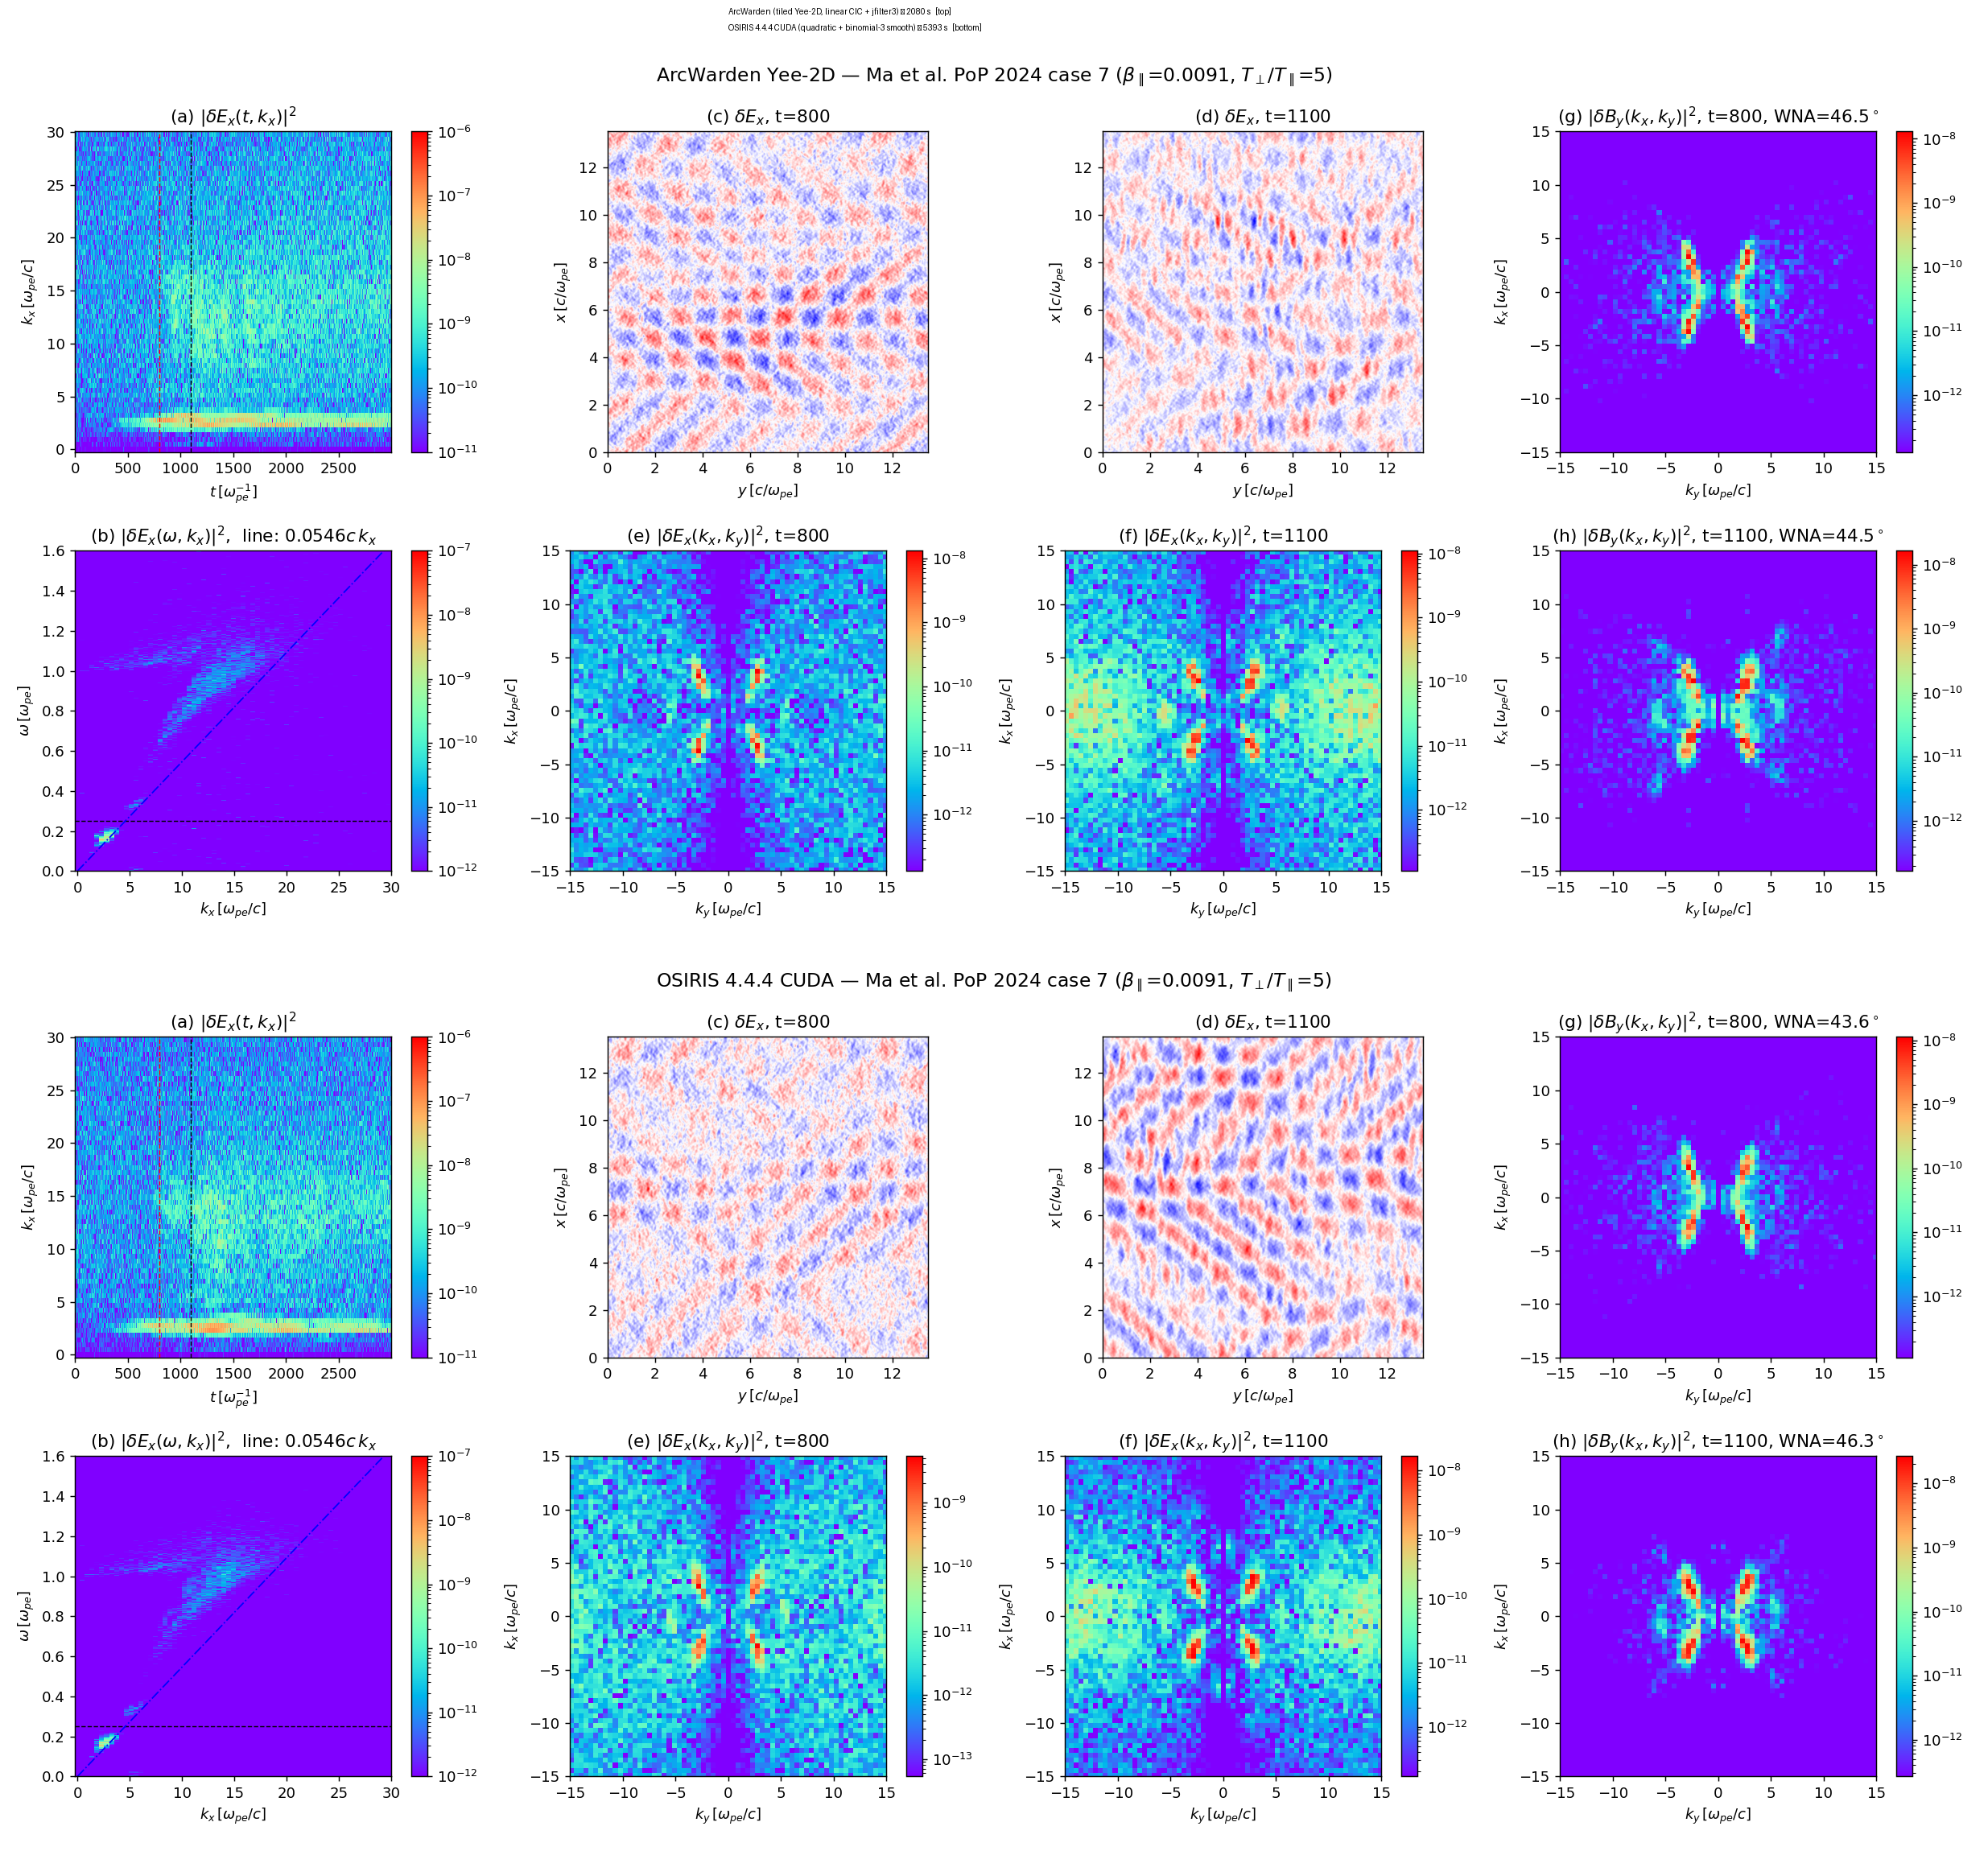
\includegraphics[width=\textwidth]{figs/eaw_case7_compare_arcwarden_osiris.png}
\caption{Case 7 of Ma et al.~\cite{ma2024} run in \arcw{} (Yee branch)
and OSIRIS-CUDA with matched diagnostics; identical eight-panel
reduction. \tocheck{final layout: possibly show 4 selected panels each}}
\label{fig:case7}
\end{figure}

\subsection{Whistler-driven nonlinear electron trapping (An et al. 2019) on
the Darwin branch}
\label{sec:an2019}
The Darwin branch is validated against the whistler-pump simulations of
An et al.~\cite{an2019} --- a like-for-like model comparison: that work
used the spectral Darwin UPIC code, i.e.\ the same magnetoinductive
field model \arcw{} implements. All three simulations of their Table~I
are reproduced from published parameters (the deck files carry the
table values verbatim): a traveling-wave pump drives a quasi-parallel
whistler; when its amplitude crosses $\delta B/B_0 \approx 0.1$,
cyclotron-resonant trapping deforms the electron distribution into a
beam and a secondary electrostatic band erupts --- Langmuir waves when
the resonant velocity is far out on the tail ($v_r = 3.2\,v_{th}$,
Sim~1), bipolar time-domain structures when it sits in the thermal bulk
($v_r \approx v_{th}$, Sim~3). \arcw{} reproduces the mechanism and the
amplitude threshold in all three cases: the electrostatic band stays at
the noise floor until $\delta B/B_0$ reaches ${\sim}0.1$ and then
erupts, at $28\times$ the floor in Sim~3 run at 268M particles
(Fig.~\ref{fig:an2019}); the phase-space panels show the chain of
trapping vortices at $v_r = 1.04\,v_{th}$ with the bipolar
$\delta E_\parallel$ signature aligned to the holes. One honest caveat:
matching the published $\delta B/B_0$ trajectory requires scaling the
pump amplitude ${\sim}5$--$6\times$ over the Table~I values (the drive
couples off our exact Darwin whistler resonance; An et al.\ likewise
tuned the drive to reach the threshold) --- the physics downstream of
the wave amplitude is parameter-free.

\begin{figure}[htbp]
\centering
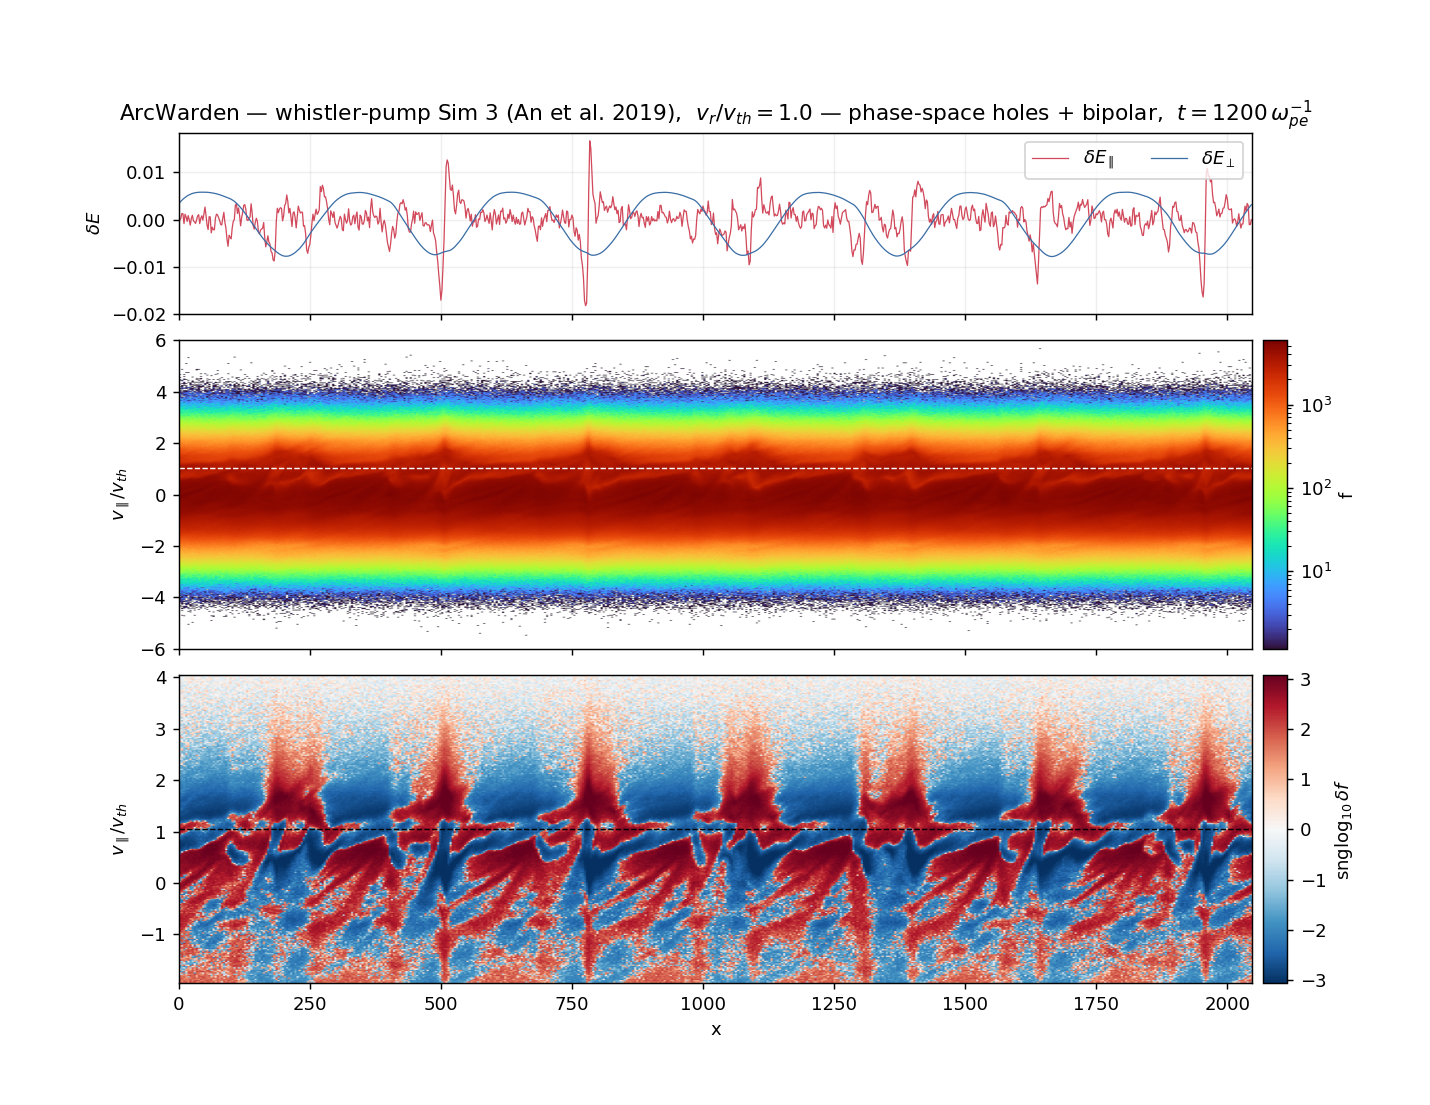
\includegraphics[width=\textwidth]{figs/whistler_s3_snap_df.png}
\caption{An et al.~\cite{an2019} Sim~3 on the Darwin branch (268M
particles): bipolar $\delta E_\parallel(x)$ (top), electron phase space
$f(x,v_\parallel)$ (middle), and signed $\delta f$ (bottom) showing the
chain of trapping vortices at the resonant velocity
$v_r = 1.04\,v_{th}$.}
\label{fig:an2019}
\end{figure}

\subsection{Chorus chirping in the electron-hybrid module}
\label{sec:hybrid}
The 1D electron-hybrid branch reproduces the rising-tone chirping
elements of Tao et al.~\cite{tao2017} from published parameters:
self-consistent generation of rising tones from an anisotropic hot
population, with the frequency sweep emerging from the nonlinear
wave--particle phase-space dynamics rather than being imposed. We
consider this the strongest integration test available for a whistler
code --- chirping is exquisitely sensitive to errors in the resonant
particle dynamics \cite{katoh2007,hikishima2009,omura2021} --- and a
result of interest in its own right, since few fresh codes have
demonstrated it (Fig.~\ref{fig:chirp}): the run shows the rising tone
in the wave spectrogram together with the resonant phase-space hole
whose upward drift in velocity is the chirping mechanism.

\begin{figure}[htbp]
\centering
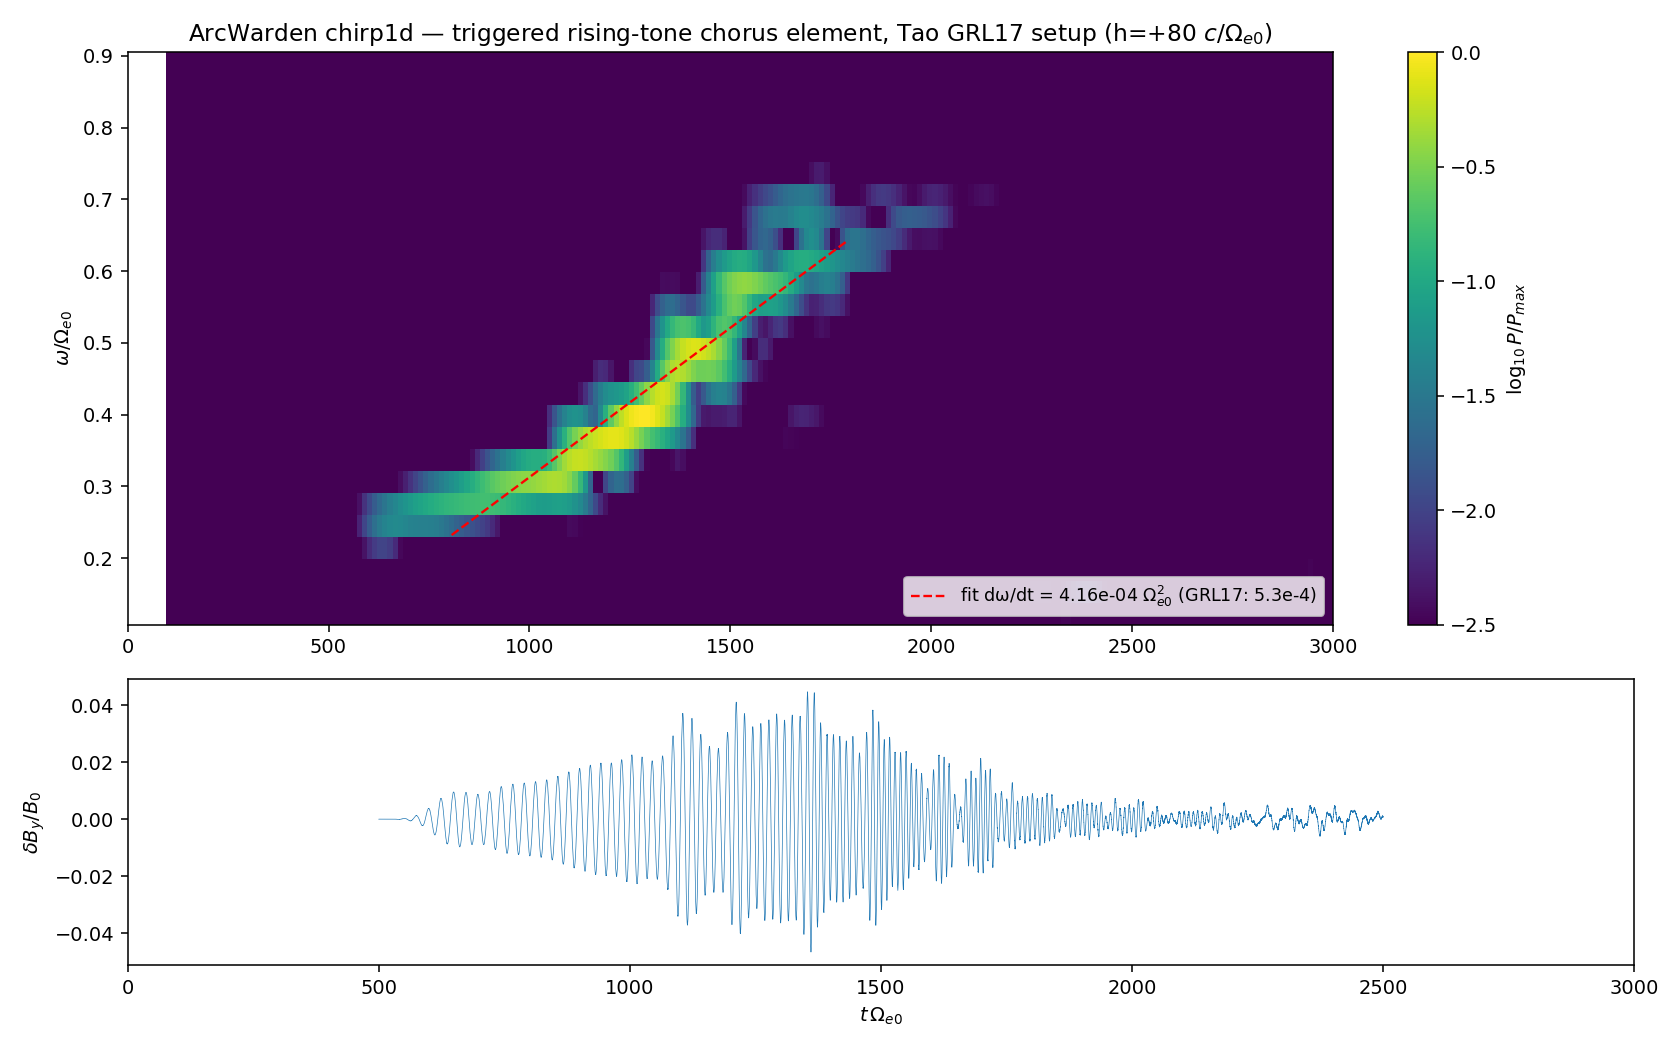
\includegraphics[width=0.72\textwidth]{figs/rising_tone_money.png}\\[2mm]
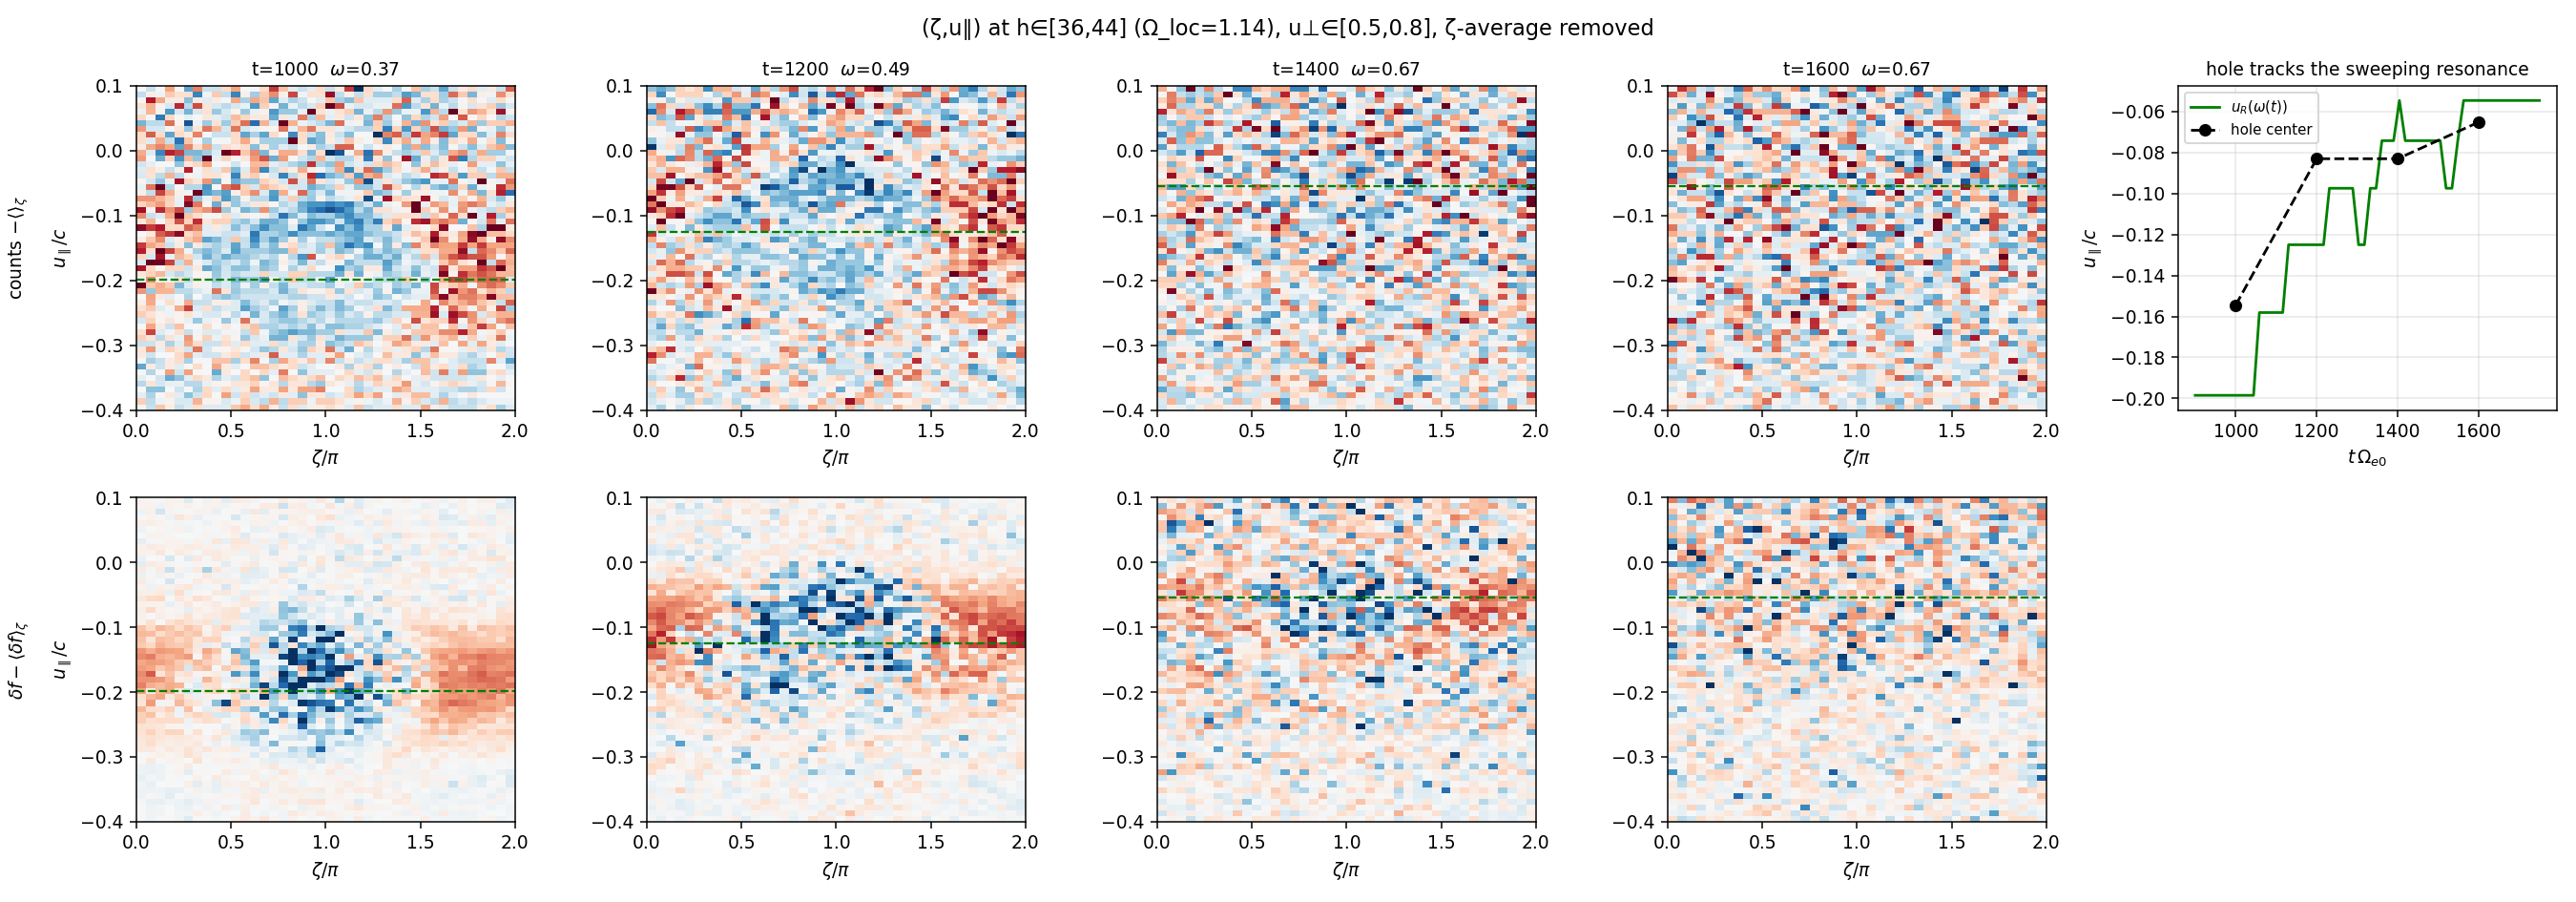
\includegraphics[width=0.72\textwidth]{figs/chirping_1d_tao_phase4_hole_tracking.png}
\caption{Electron-hybrid branch, Tao et al.~2017 setup. Top: rising-tone
spectrogram of the self-consistently generated chorus element. Bottom:
tracking of the resonant phase-space hole that drives the frequency
sweep. \tocheck{final figure selection/cropping}}
\label{fig:chirp}
\end{figure}

\subsection{Cross-branch validation}
\label{sec:crossbranch}
The Darwin and Yee branches are validated against each other in the
low-frequency regime where the Darwin approximation holds
($\omega^2 \ll k^2c^2$); agreement between a radiation-free spectral
solver and a full-Maxwell FDTD solver sharing only the particle engine
is a sensitive check on both. Two levels:

\emph{Eigenmode level} (continuous-integration gate): a cold-plasma
parallel whistler at $kc = 3\,\omega_{pe}$, $\omega_{ce} =
0.5\,\omega_{pe}$ is seeded identically in both branches and its
frequency measured from the identical particle-current projection. The
Darwin branch measures $\omega = 0.44980$ against its analytic
dispersion $0.45000$ (0.05\%); the Yee branch measures $0.44885$
against the full-Maxwell root $0.44897$ (0.03\%); and the 0.21\% gap
\emph{between} the two measured frequencies matches the 0.23\% analytic
displacement-current gap between the models --- the two branches differ
by exactly the physics that separates the field models. The same gate
bounds the Yee branch's running conservation residuals: $\nabla\cdot B$
identically zero to round-off, and the Gauss residual
$\nabla\cdot E - \rho$ frozen at its initial value to
${\sim}2\times10^{-7}$ (the Esirkepov guarantee).

\emph{Nonlinear level}: An et al.\ Sim~3 (Sec.~\ref{sec:an2019}) was
re-run through the Yee branch with the same deck (at the light-CFL time
step, $6.25\times$ more steps). The whistler amplitude histories peak
at $\delta B/B_0 = 0.105$ (Darwin) vs $0.108$ (Yee) with an identical
kinetic ring-down, and the nonlinear electrostatic band and phase-space
trapping structures agree (Fig.~\ref{fig:crossbranch}).

\begin{figure}[htbp]
\centering
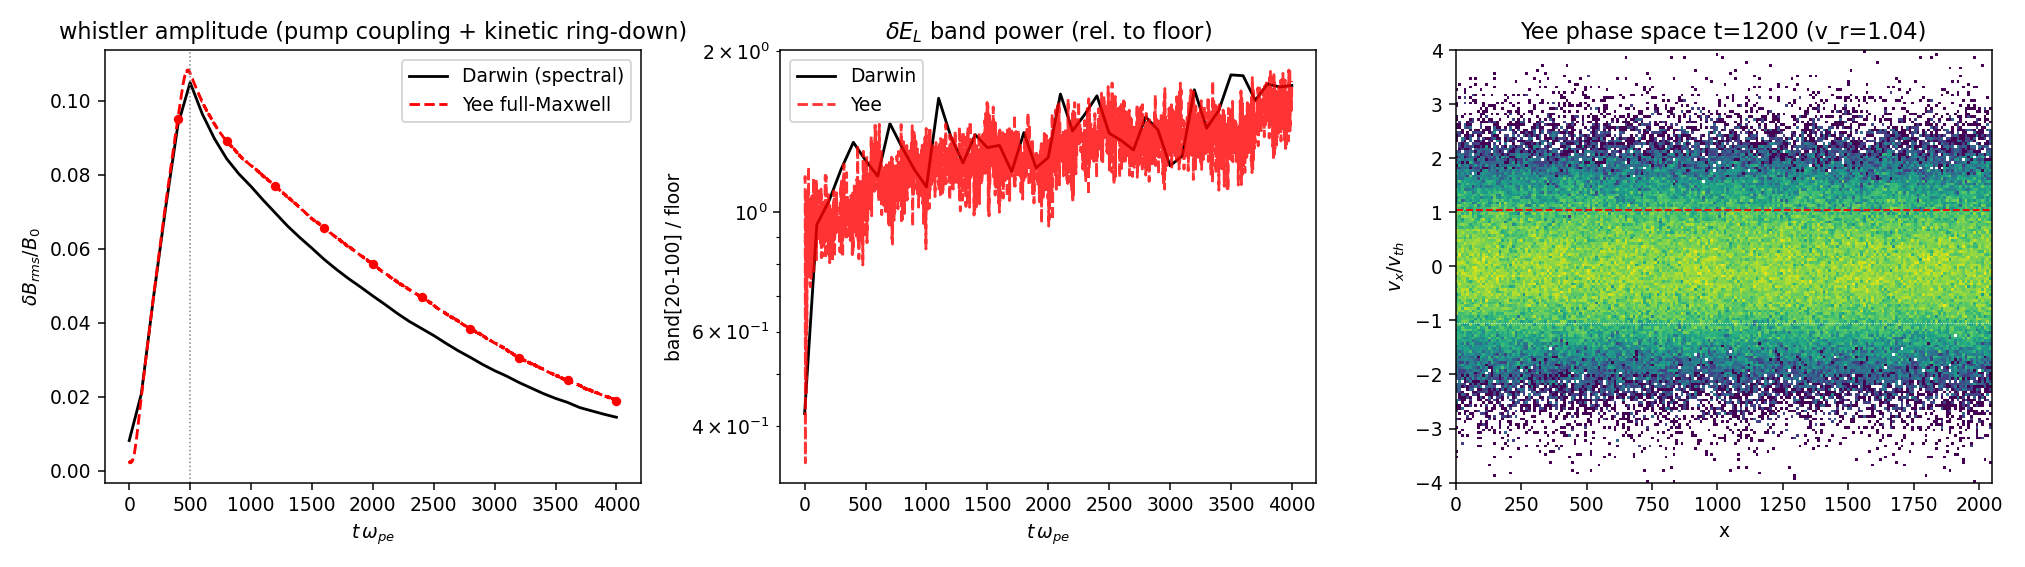
\includegraphics[width=\textwidth]{figs/an_cross_check.png}
\caption{Darwin (spectral) vs Yee (full-Maxwell) on the An et al.\
Sim~3 deck: whistler amplitude history (left; peaks 0.105 vs 0.108),
secondary electrostatic band power relative to the noise floor
(middle), and the Yee-branch phase space at $t=1200\,\omega_{pe}^{-1}$
(right).}
\label{fig:crossbranch}
\end{figure}

%=====================================================================
\section{Performance}
\label{sec:perf}

\subsection{Head-to-head against OSIRIS-CUDA}
\label{sec:headtohead}
Table~\ref{tab:headtohead} shows the headline result: the identical
case-7 problem, both codes on the same RTX~5090, both writing the
matched diagnostic set (six-field 2D dumps every $50\,\omega_{pe}^{-1}$,
lineouts every $1\,\omega_{pe}^{-1}$), figures produced by the same
analysis pipeline.

\begin{table}[htbp]
\centering
\caption{Case-7 end-to-end wall time, matched physics and diagnostics.
156.25M particles, 206{,}897 steps, RTX 5090.}
\label{tab:headtohead}
\begin{tabular}{lccc}
\toprule
code & wall time & particle-steps/s & speedup\\
\midrule
OSIRIS 4.4.4 CUDA (quadratic, binomial-3) & \SI{5392.8}{s} & $6.0\times10^{9}$ & 1\\
\arcw{} Yee tiled (linear, binomial-3)     & \SI{2079.7}{s} & $1.55\times10^{10}$ & $2.59\times$\\
\bottomrule
\end{tabular}
\end{table}

The interpolation orders differ (quadratic is OSIRIS's production
configuration for this problem; \arcw{} is linear+filter) --- but
Section~\ref{sec:overhead} shows by direct measurement that
interpolation order is nearly free in the OSIRIS-CUDA rate (7\%), so the
comparison is dominated by architecture, not arithmetic.
\tocheck{optional: implement quadratic in the tiled framework
(est. 20--30\% cost) and quote exact-shape-parity numbers}

\subsection{Ablation: where the speedup comes from}
\label{sec:ablation}
Table~\ref{tab:ablation} isolates each design element on the case-7
configuration with diagnostics disabled.

\begin{table}[htbp]
\centering
\caption{Ablation chain, case-7 configuration, no diagnostics.}
\label{tab:ablation}
\begin{tabular}{lcc}
\toprule
configuration & particle-steps/s & gain\\
\midrule
flat: fused kernel, global-atomic Esirkepov & $4.5\times10^{9}$ & ---\\
+ $16{\times}16$ tile sort (every 20) + shared apron deposit & $1.51\times10^{10}$ & $3.4\times$\\
+ migration fused into scatter write-back & $1.61\times10^{10}$ & $+6.6\%$\\
\bottomrule
\end{tabular}
\end{table}

Two supporting microbenchmarks: the tiled charge deposit alone is
$6.4\times$ faster than global atomics (14.9 vs 2.3~Gdep/s), and the
plain L2-served push runs at 35.4~Gpush/s --- while a shared-memory
field-staging variant of the same push measures $0.82\times$, the
negative result that motivates design rule~1. Sort cadence is a flat
dial: $N_{\rm sort}=10/20/40$ gives $1.45/1.51/1.54\times10^{10}$.

\subsection{The classic design is overhead-bound on this hardware}
\label{sec:overhead}
Three independent measurements on the OSIRIS-CUDA reference:
\begin{enumerate}
\item \textbf{GPU utilization is 52\%} during the production run
  (sampled over minutes, no diagnostics window) --- nearly half the
  device is idle between pipeline stages.
\item \textbf{Interpolation order is nearly free.} Switching
  linear$\to$quadratic ($\sim2\times$ the deposit arithmetic and
  $2.25\times$ the stencil) moves the rate only from
  $6.3$ to $5.9\times10^{9}$ ($-7\%$). A compute-bound code cannot do
  this.
\item \textbf{Chunk size is an exact null.} Doubling
  \texttt{chunk\_size} from 512 to 1024 particles (halving the number of
  chunk-pipeline work items) leaves the rate at $5.92\times10^{9}$ in
  both cases. The cost is the per-step find-movers/exchange/compact
  pipeline itself --- proportional to particles and pipeline stages, not
  to chunk granularity.
\end{enumerate}
Together these identify per-step particle bookkeeping as the pacing
item of the classic design on cache-rich hardware, which is precisely
the term \arcw{} deletes (Section~\ref{sec:design-deposit}).

\subsection{The Darwin branch: time-to-solution on one GPU}
\label{sec:darwin}
The Darwin branch runs the same case-7-scale problem ($625^2$, 156.25M
particles) at $\Delta t = 0.1\,\omega_{pe}^{-1}$ --- $6.9\times$ the Yee
light-CFL step. Its measured end-to-end rate is $5.0\times10^{9}$
particle-steps/s (\SI{31.4}{ms} per step, marginal over 400 steps,
2026-07-16), so the full case-7 physical time
($t=3000\,\omega_{pe}^{-1}$, i.e.\ 30{,}000 Darwin steps) costs
$\approx\SI{943}{s}$. Per unit of \emph{physical time simulated}, the
Darwin branch is therefore $2.2\times$ cheaper than the (already
$2.6\times$-accelerated) tiled Yee branch and $5.7\times$ cheaper than
the OSIRIS-CUDA reference, on problems whose physics it captures, at
the price of excluding light waves and $O(\omega^2/k^2c^2)$
corrections. This is the practical sense in which a radiation-free
solver is ``very good for one GPU'': the model buys a larger factor
than any kernel optimization, and it \emph{stacks} with them. The
branch sustains 98--100\% GPU utilization at $\approx$\SI{485}{W}
(sampled with \texttt{nvidia-smi} during the benchmark) --- against the
52\% of the chunk-pipeline reference.

The kernel-level profile (Table~\ref{tab:darwinstep}) also quantifies
the branch's known headroom: it still guarantees tile locality the old
way, sorting \emph{every} step --- the design the Yee branch abandoned
in Section~\ref{sec:design-deposit} --- spending \SI{11.6}{ms} of the
\SI{31.4}{ms} step on the sort plus \SI{2.1}{ms} on a separate
migration kernel. Applying the already-validated amortized
stale-tolerant sort and fused migration projects the step to
$\approx\SI{18}{ms}$ ($8.7\times10^{9}$ particle-steps/s,
$\approx\SI{550}{s}$ for the case-7-equivalent physical time, i.e.\
$\approx10\times$ the reference end-to-end); the shared-apron scatter
applied to the three moment deposits would add more.
\tocheck{implement and replace projections with measurements; also run
a physics case (e.g. whistler growth) on both branches for a
same-figure Darwin-vs-Yee panel}

\begin{table}[htbp]
\centering
\caption{Darwin-branch per-step kernel budget at case-7 scale
(Nsight Systems averages over 300 steps, RTX 5090). The entire
spectral field solve --- all cuFFTs plus $k$-space kernels --- totals
$<0.2$\,ms.}
\label{tab:darwinstep}
\begin{tabular}{lcc}
\toprule
kernel & ms/step & share\\
\midrule
per-step tile sort (legacy; to be amortized) & 11.6 & 36\%\\
fused gather + Boris push & 8.0 & 25\%\\
$\rho$+$J$ tiled deposit & 3.4 & 11\%\\
$\langle uu\rangle$ (amu) moment deposit & 3.3 & 10\%\\
$\dot J$ (dcu) moment deposit & 3.0 & 9\%\\
migration (legacy; fused into scatter in the Yee branch) & 2.1 & 7\%\\
spectral solves (all cuFFT + $k$-space kernels) & 0.17 & 0.5\%\\
\bottomrule
\end{tabular}
\end{table}

\subsection{Profiling}
\label{sec:profiling}
Nsight Systems timelines for both branches accompany the repository
(\texttt{profiling/}). The Yee-branch kernel summary quantifies the
design directly: the fused particle kernel is 87.7\% of all GPU time
(median \SI{9.3}{ms} per step); the amortized sort contributes
\SI{0.64}{ms} per step (12.1\,ms every 20 steps); and the entire
Maxwell update --- two Faraday half-steps, one Amp\`ere step, and nine
binomial filter passes --- totals $\approx\SI{0.05}{ms}$ per step
(0.5\%). During the same benchmark the device sustains 100\% GPU
utilization at $\approx$\SI{575}{W} (1 Hz \texttt{nvidia-smi} samples;
the Darwin branch reads 98--100\% at $\approx$\SI{485}{W}) --- against
52\% for the chunk-pipeline reference on the identical problem. The
GPU therefore spends essentially all of its time on the irreducible
particle work, which is the design goal stated in
Section~\ref{sec:design-hw}. \tocheck{ncu kernel report
(profiling/collect\_ncu.sh, needs perf-counter permission): quote SOL
memory/compute \%, achieved occupancy, and the L2 hit rate of the
field gathers}

%=====================================================================
\section{Discussion and limitations}
\label{sec:discussion}
\begin{itemize}
\item \textbf{Scope of the L2 argument.} The design rule ``fields live in
  L2'' holds for 2D electron-scale grids up to roughly $1600^2$--$2000^2$
  on a \SI{96}{MB} device (nine single-precision arrays --- six gathered
  field components plus three scattered current components --- or six if
  only the gathers need residency). For larger
  grids or 3D, the gather working set exceeds L2 and tile-locality of
  \emph{field reads} becomes valuable again --- but via the same
  amortized sort already present, not via per-step chunk bookkeeping.
  The stale-tolerant-sort result is the part we expect to transfer
  unchanged to any architecture.
\item \textbf{Single GPU, single precision, 2D3V.} All results here are
  one GPU. Multi-GPU domain decomposition (planned along with the
  dipole-field L-shell extension) reintroduces halo exchange; the fused
  kernel is compatible with it because the stray fallback already
  tolerates out-of-tile particles.
\item \textbf{Comparison fairness.} OSIRIS ran its production
  configuration (quadratic), \arcw{} linear+filter; the overhead-bound
  measurements (Section~\ref{sec:overhead}) bound the effect of this
  difference at $\sim$7\% of the OSIRIS rate. A quadratic tiled deposit
  is straightforward in the \texttt{Sink} framework and is the cleanest
  way to close the gap entirely. \tocheck{decide before submission}
\item \textbf{Consumer vs datacenter hardware.} The RTX~5090 is a
  \$2k-class consumer device; the result that a full 156M-particle,
  207k-step kinetic run finishes in 35 minutes on it is itself a
  statement about the accessibility of electron-scale kinetics.
  Datacenter Blackwell (B200) has yet larger L2 and HBM; nothing in the
  design depends on consumer-specific features.
\end{itemize}

%=====================================================================
\section{Development methodology: pair-programming with an LLM agent}
\label{sec:methodology}
\arcw{} was developed by one physicist working with an LLM coding agent
(Claude Code, Anthropic) over a series of sessions, under explicit,
human-written rules. We document the working rules because we found the
discipline --- not the raw code generation --- to be the determinant of
whether agent-written GPU code can be trusted:

\begin{enumerate}
\item \textbf{A plan with milestones and quantitative gates.} The
  project runs on a written plan (M0--M12) in which every milestone has
  an acceptance gate stated \emph{before} the work: e.g.\ the tiled
  deposit (M9) required a charge-conservation residual $<2\times10^{-4}$
  with a deliberately stale sort, and an end-to-end rate target, before
  merging. The agent is not permitted to declare a milestone done; the
  gate is.
\item \textbf{Tests precede performance.} Every optimization lands
  behind a \texttt{ctest}: J-identity, continuity, energy parity
  (Section~\ref{sec:design-gates}). This caught real agent errors ---
  including a test harness that violated the light CFL and the
  $\omega_{pe}\Delta t$ stability limits simultaneously, producing
  failures unrelated to the code under test; the debugging that followed
  (three distinct stability violations, fixed in sequence) is exactly
  the physics reasoning a domain scientist must supply.
\item \textbf{A committed performance baseline.} Every kernel change is
  measured against a versioned baseline document
  (\texttt{docs/PROFILE\_BASELINE.md}); ``it should be faster'' is not
  accepted, and negative results (the $0.82\times$ shared-field push)
  are recorded rather than discarded --- one such negative result became
  design rule~1 of this paper.
\item \textbf{Published figures as acceptance tests.} Milestones close
  by reproducing a published figure (Tao et al.\ 2017 chirping;
  Ma et al.\ 2024 Fig.~1) from published parameters, not by unit tests
  alone. This is the only test class that exercises every term at once.
\item \textbf{Run data are never deleted by the agent.} A standing rule:
  simulation outputs are moved aside, never removed, after plotting ---
  re-running a 35-minute (or 90-minute) case to regenerate a figure is
  the most expensive class of agent mistake.
\item \textbf{Persistent memory across sessions.} The agent maintains
  a memory of the project state, verified parameters from the
  literature, and previously-made decisions, so that each session
  resumes from the plan rather than from zero.
\end{enumerate}

Two observations for the community. First, the agent's throughput moved
the bottleneck to \emph{verification}: the human role concentrated into
writing gates, judging physics plausibility, and catching
stability-limit violations --- all domain knowledge, none of it
mechanical. Second, the milestone-gate structure turned out to be what
makes the collaboration compounding rather than chaotic: the plan
document, the baseline document, and the test suite are the interfaces
through which human intent constrains agent freedom, and we would
recommend exactly those three artifacts to any group attempting the
same. The full development history is preserved in the repository's
commit log and planning documents.

%=====================================================================
\section{Conclusions}
\label{sec:conclusions}
A PIC code designed around what modern GPUs actually provide ---
cache-resident fields, fused step kernels, shared-memory scatter aprons,
and amortized, stale-tolerant sorting in place of per-step particle
bookkeeping --- outperforms the classic chunk-pipeline GPU-PIC design by
$2.6\times$ on identical physics on the same device, and we can account
for the gain element by element. The same particle engine hosts a
radiation-free Darwin solver whose $6.9\times$ larger time step buys a
further $2.2\times$ in time-to-solution today (with measured headroom to
$\sim$$4\times$ once its legacy per-step sort adopts the amortized
scheme) for the low-frequency electromagnetic problems that dominate
inner-magnetosphere physics --- and that reproduces the published
spectral-Darwin trapping results of An et al.~\cite{an2019} from their
parameters --- and an
electron-hybrid module that reproduces chorus chirping from published
parameters. Electron-scale kinetic runs that were cluster jobs are now
half-hour desktop jobs on consumer hardware; we believe the design
rules, the stale-tolerant sort in particular, transfer directly to the
exascale codes.

\section*{Acknowledgments}
Development used Claude Code (Anthropic) under the methodology of
Section~\ref{sec:methodology}. \tocheck{grants, computing, colleagues}

\section*{Code and data availability}
\arcw{} is available at \tocheck{repository URL on publication}. Run
decks, analysis scripts, profiling reports, and the OSIRIS input files
used for the comparison are included in the repository.

\bibliographystyle{unsrt}
\bibliography{refs}

\end{document}
